% !TeX root = ../../../book.tex

\subsection{函数复合}

\subsubsection*{引言}

让我们来思考一下函数的示意图。假设我们有一个函数 $f : A \to B$,还有一个函数 $g : B \to C$,它们的定义如下:

\begin{multicols}{2}
    \begin{center}
        {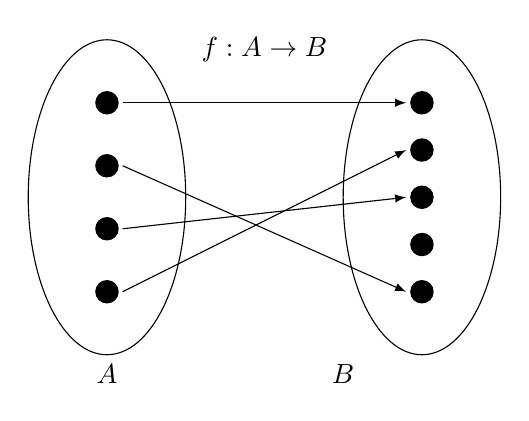
\begin{tikzpicture}[scale=1]
                \foreach \x in {0,...,4}
                    {
                        \node at (4, -\x*0.6)[circle,fill,inner sep=3pt]{};
                    }
                \draw (4,-1.2) ellipse (1 and 2);

                \foreach \x in {0,...,3}
                    {
                        \node at (0, -\x*0.8)[circle,fill,inner sep=3pt]{};
                    }
                \draw (0,-1.2) ellipse (1 and 2);

                \draw[-latex] (0.2,-0.0) -- (3.8,0.0);
                \draw[-latex] (0.2,-0.8) -- (3.8,-2.4);
                \draw[-latex] (0.2,-1.6) -- (3.8,-1.2);
                \draw[-latex] (0.2,-2.4) -- (3.8,-0.6);

                \node[below] at (0, -3.2){$A$};
                \node[below] at (3, -3.2){$B$};
                \node[above] at (2, 0.4){$f:A \to B$};
            \end{tikzpicture}}
    \end{center}

    \begin{center}
        {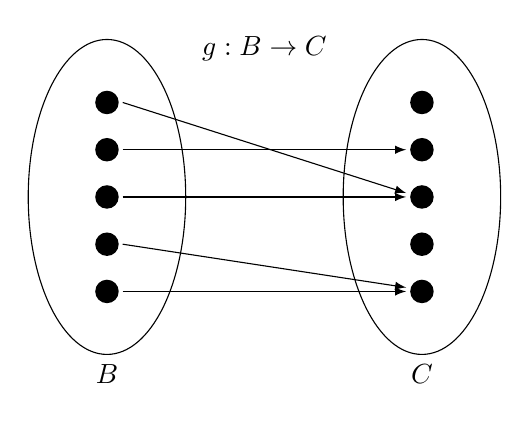
\begin{tikzpicture}[scale=1]
                \foreach \x in  {0,...,4}
                    {
                        \node at (4, -\x*0.6)[circle,fill,inner sep=3pt]{};
                    }
                \draw (4,-1.2) ellipse (1 and 2);

                \foreach \x in  {0,...,4}
                    {
                        \node at (0, -\x*0.6)[circle,fill,inner sep=3pt]{};
                    }
                \draw (0,-1.2) ellipse (1 and 2);

                \draw[-latex] (0.2,-0.0) -- (3.8,-1.15);
                \draw[-latex] (0.2,-0.6) -- (3.8,-0.6);
                \draw[-latex] (0.2,-1.2) -- (3.8,-1.2);
                \draw[-latex] (0.2,-1.8) -- (3.8,-2.35);
                \draw[-latex] (0.2,-2.4) -- (3.8,-2.4);

                \node[below] at (0, -3.2){$B$};
                \node[below] at (4, -3.2){$C$};
                \node[above] at (2, 0.4){$g:B \to C$};
            \end{tikzpicture}}
    \end{center}
\end{multicols}

直观感觉,$f$ 就像一张``地图'',为我们提供了从 $A$ 中元素到 $B$ 中元素的特定路线,而 $g$ 则是从 $B$ 中元素到 $C$ 中元素的``地图''。如果我们依次遵循这些``地图'',会发生什么呢?也就是说,让我们把这两张``地图''叠加起来,

\begin{center}
    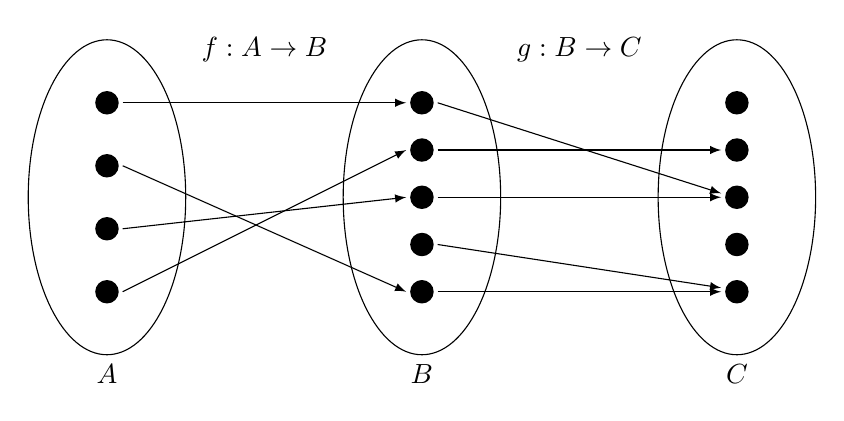
\begin{tikzpicture}[scale=1]
        \foreach \x in {0,...,3}
            {
                \node at (0, -\x*0.8)[circle,fill,inner sep=3pt]{};
            }
        \draw (0,-1.2) ellipse (1 and 2);

        \foreach \x in {0,...,4}
            {
                \node at (4, -\x*0.6)[circle,fill,inner sep=3pt]{};
            }
        \draw (4,-1.2) ellipse (1 and 2);

        \foreach \x in  {0,...,4}
            {
                \node at (8, -\x*0.6)[circle,fill,inner sep=3pt]{};
            }
        \draw (8,-1.2) ellipse (1 and 2);

        \draw[-latex] (0.2,-0.0) -- (3.8,0.0);
        \draw[-latex] (0.2,-0.8) -- (3.8,-2.4);
        \draw[-latex] (0.2,-1.6) -- (3.8,-1.2);
        \draw[-latex] (0.2,-2.4) -- (3.8,-0.6);

        \draw[-latex] (4.2,-0.0) -- (7.8,-1.15);
        \draw[-latex] (4.2,-0.6) -- (7.8,-0.6);
        \draw[-latex] (4.2,-1.2) -- (7.8,-1.2);
        \draw[-latex] (4.2,-1.8) -- (7.8,-2.35);
        \draw[-latex] (4.2,-2.4) -- (7.8,-2.4);

        \node[below] at (0, -3.2){$A$};
        \node[below] at (4, -3.2){$B$};
        \node[below] at (8, -3.2){$C$};
        \node[above] at (2, 0.4){$f:A \to B$};
        \node[above] at (6, 0.4){$g:B \to C$};
    \end{tikzpicture}
\end{center}

然后直接从 $A$ 到 $C$,省略中间环节:

\begin{center}
    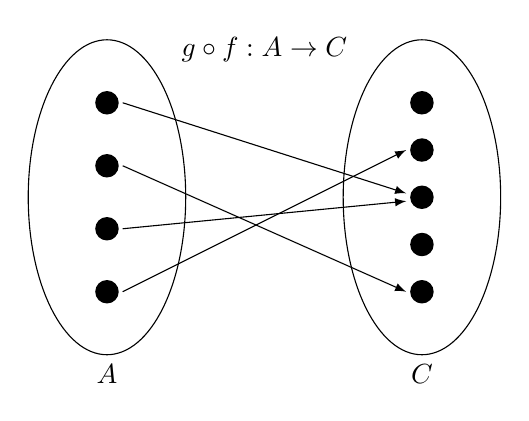
\begin{tikzpicture}[scale=1]
        \foreach \x in {0,...,4}
            {
                \node at (4, -\x*0.6)[circle,fill,inner sep=3pt]{};
            }
        \draw (4,-1.2) ellipse (1 and 2);

        \foreach \x in {0,...,3}
            {
                \node at (0, -\x*0.8)[circle,fill,inner sep=3pt]{};
            }
        \draw (0,-1.2) ellipse (1 and 2);

        \draw[-latex] (0.2,-0.0) -- (3.8,-1.15);
        \draw[-latex] (0.2,-0.8) -- (3.8,-2.4);
        \draw[-latex] (0.2,-1.6) -- (3.8,-1.25);
        \draw[-latex] (0.2,-2.4) -- (3.8,-0.6);

        \node[below] at (0, -3.2){$A$};
        \node[below] at (4, -3.2){$C$};
        \node[above] at (2, 0.4){$g \circ f:A \to C$};
    \end{tikzpicture}
\end{center}

这看起来是个合理的做法,对吧?当然是的!每当我们有数学对象时,我们总是好奇如何合理地组合、操作和泛化它们。在函数的情况下,我们称这种组合为函数的\textbf{复合}。你可能会注意到,只有当``第一个''函数的值域与``第二个''函数的定义域相同时,这种复合才有意义。这一点在下面的定义中有所体现。

\subsubsection*{定义}

\begin{definition}
    设 $A, B, C$ 为集合,$f : A \to B$ 和 $g : B \to C$ 为函数。考虑函数 $h : A \to C$ 定义为:
    \[\forall a \in A \centerdot h(a) = g(f(a))\]
    我们说 $h$ 是 $g$ 和 $f$ 的\dotuline{复合},写做 $g \circ f$。

    我们也可以将该术语简化为 $f$ 是 ``$g$ 复合 $f$''。
\end{definition}

这结合了我们之前提到的所有概念。要求函数 $f$(``第一个''函数)的值域必须是函数 $g$(``第二个''函数)的定义域。

我们可以将函数直观地理解为一台\emph{机器}或一个\emph{黑箱}。输入定义域中的元素,输出值域中的元素。我们不一定知道机器内部的具体操作,只能看到输出结果。现在,想象将两台机器连接起来,一台执行 $f$,一台执行 $g$;将 $f$ 机器的输出作为 $g$ 机器的输入。最终的输出是集合 $C$ 中的一个元素。我们可以把这两台机器看作是一台更大的机器。这就是\emph{复合} $g \circ f$ 的作用;它相当于一台更大的机器,按特定顺序执行两台机器的操作。

\subsubsection*{符号}

注意符号 $g \circ f$ 的顺序以及它与我们应用函数顺序的对比:先应用 $f$,然后是 $g$,即 $g(f(a))$。用语言描述,我们会将``$g(f(a))$'' 读作 ``$a$ 的 $f$ 的 $g$''。事实上,如果你发现自己难以记住这个顺序,这里有一个建议:将 “$\circ$” 读作 ``在……之后''。因此,$h = g \circ f$ 意味着 ``$g$ 在 $f$ 之后'',因为我们先对 $a$ 元素应用 $f$,然后再应用 $g$。

记住复合函数的符号也很重要,并且要区分函数 $g \circ f$ 本身和将某元素 $x \in A$ 应用于函数 $g \circ f$。例如,要使用 ``$\circ$'' 符号表示``$x$ 的 $f$ 的 $g$'',我们会写
\[(g \circ f)(x)\]
因为我们将函数 $g \circ f$ 应用于元素 $x$。然而,以下符号是\textbf{没有意义的},因为它混淆了函数和元素的概念:
\[g \circ f(x)\]
你能看出区别吗?$f(x)$ 是集合 $B$ 中的一个元素,$B$ 是 $f$ 的值域。但 $g$ 是一个函数。将函数与集合中的元素复合是什么意思?这行不通。通常来说,要注意这一点!当我们必须将多个函数复合在一起时,这种区别尤其重要,例如 $(h \circ (g \circ k) \circ f)(z)$,其中 $z$ 是 $f$ 定义域中的元素,而 $f,g,h,k$ 都是函数。

\subsubsection*{示例}

\begin{example}
    定义函数 $ C : \mathbb{R} \to \mathbb{R}$ 为
    \[\forall x \in \mathbb{R} \centerdot C(x) = x - 273.15\]

    定义函数 $ F : \mathbb{R} \to \mathbb{R}$ 为
    \[\forall x \in \mathbb{R} \centerdot F(x) = \frac{9}{5}x + 32\]

    函数 $C$ 将开尔文温度转换为摄氏温度。

    函数 $F$ 将摄氏温度转换为华氏温度。

    函数 $F \circ C$ 直接将开尔文温度转换为华氏温度。我们可以复合函数的``规则''从而找到直接转换的公式。
    \begin{align*}
        \forall x \in \mathbb{R} \centerdot (F \circ C)(x) & = F(C(x)) = F(x - 273.15)                                  \\
                                                           & = \frac{9}{5} \cdot (x - 273.15) + 32 = \frac{9}{5}-459.67
    \end{align*}
\end{example}

\begin{example}
    设函数 $f : \mathbb{R} \to \mathbb{Z}$ 定义为
    \[\forall x \in \mathbb{R} \centerdot f(x) = \lfloor x \rfloor\]
    ($\lfloor x \rfloor$ 表示 $x$ 向下取整:即满足 $z \le x$ 的\emph{最大}整数 $z \in \mathbb{Z}$。)

    设函数 $g : \mathbb{Z} \to \mathbb{N}$ 定义为
    \[\forall z \in \mathbb{Z} \centerdot g(z) = \begin{cases}
            -z  & \text{如果}\;z<0     \\
            z+1 & \text{如果}\;z \ge 0
        \end{cases}\]

    我们来找出 $g \circ f$。

    注意,只要 $x \in \mathbb{R} < 0$,我们都可以得到 $\lfloor x \rfloor < 0$。同理,只要 $x \in \mathbb{R} \ge 0$,我们都可以得到 $\lfloor x \rfloor \ge 0$。这告诉我们 $g \circ f$ 是一个\textbf{分段}函数:
    \[\forall x \in \mathbb{R} \centerdot (g \circ f)(x) = \begin{cases}
            -\lfloor x \rfloor  & \text{如果}\;z<0     \\
            \lfloor x \rfloor+1 & \text{如果}\;z \ge 0
        \end{cases}\]
    问题:这个函数是单射吗?是满射吗?试着证明你的结论。
\end{example}

\begin{example}
    定义函数 $f : \mathbb{N} \to \mathbb{N}, g : \mathbb{Z} \to \mathbb{N}, h : \mathbb{Z} \to \mathbb{N}$ 为:
    \begin{align*}
        \forall n \in \mathbb{N} \centerdot f(n) & = n + 3  \\
        \forall n \in \mathbb{N} \centerdot g(n) & = n^2    \\
        \forall n \in \mathbb{N} \centerdot h(n) & = 2n - 1
    \end{align*}
    (问题:你确定这些函数都是良好定义的吗?为什么?)

    我们可以找到 $g \circ f$ 和 $h \circ g$ 的``规则'':
    \begin{align*}
        \forall n \in \mathbb{N} \centerdot (g \circ f)(n) & = g(f(n)) = g(n + 3) = (n + 3)^2 = n^2 + 6n + 9 \\
        \forall n \in \mathbb{N} \centerdot (h \circ g)(n) & = h(g(n)) = h(n^2) = 2n^2-1
    \end{align*}

    我们可以由此得到进一步复合的规则,比如 $h \circ (g \circ f)$:
    \begin{align*}
        \forall n \in \mathbb{N} \centerdot \big(h \circ (g \circ f)\big)(n) & = h\big((g \circ f)(n)\big) = h(n^2 + 6n + 9) \\
                                                                             & = 2(n^2 + 6n + 9) - 1                         \\
                                                                             & = 2n^2 + 12n + 17
    \end{align*}

    类似地,我们可以找到 $(h \circ g) \circ f$ 的规则:
    \begin{align*}
        \forall n \in \mathbb{N} \centerdot \big((h \circ g) \circ f\big)(n) & = (h \circ g)(f(n)) = (h \circ g)(n + 3) \\
                                                                             & = 2(n + 3)^2 - 1 = 2(n^2 + 6n + 9) - 1   \\
                                                                             & = 2n^2 + 12n + 17
    \end{align*}
\end{example}

看一下上面两个结果,他们是相等的!也就是说,从\emph{函数}意义上讲,我们刚刚通过证明在\emph{每一个}允许的输入上都能产生相同的输出,从而\emph{证明}了
\[h \circ (g \circ f) = (h \circ g) \circ f\]

\subsubsection*{复合结合律}

在前面的例子中,函数 $f, g, h$ 并没有什么特别之处。实际上,我们得到的结果在\emph{一般情况下}都是成立的。下面的定理和证明将表明这一点。我们要证明的是函数复合满足\textbf{结合律}。这意味着在进行多重函数复合时,可以随意移动括号,而不影响结果。

\begin{theorem}
    设 $A,B,C D$ 为任意集合。设 $f : A \to B, g : B \to C, h : C \to D$ 为函数。则
    \[h \circ (g \circ f) = (h \circ g) \circ f\]
\end{theorem}

\begin{proof}
    我们要证明对于任意可能的输入,函数 $(h \circ g) \circ f$ 和函数 $h \circ (g \circ f)$ 的输出相同。

    给定 $x \in A$,应用\emph{复合}的定义,可得
    \[[h \circ (g \circ f)](x) = h\big((g \circ f)(x)\big) = h\big(g(f(x))\big)\]
    且
    \[[(h \circ g) \circ f](x) = \big(h \circ g\big)(f(x)) = h\big(g(f(x))\big)\]
\end{proof}

\subsubsection*{复合与映射}

现在有一个有趣的问题:如果我们将两个具有相同性质的函数复合起来,会发生什么?这个性质依然存在吗?比如,如果我们复合两个单射函数,结果还是单射函数吗?是否只需要其中一个函数是单射,就能确保复合后的函数也是单射?

同理,假设我们有两个函数的复合。如果已知复合后的函数是满射,我们能否确定其中一个函数也是满射?还是说两个函数都必须是满射?

在这部分内容中,我们将陈述并证明一些关于这些问题的结论。我们也会让你在本节和本章末尾的练习中证明一些相关的事实,或者找到适当的反例。

\begin{proposition}
    设 $A, B, C$ 为集合,$f : A \to B$ 和 $g : B \to C$ 为函数。如果 $g \circ f$ 为单射,则 $f$ 必为单射。
\end{proposition}

(请注意,这里并不假设 $g$ 具有任何特定性质;$g$ 甚至不一定是单射!作为练习,试着找出函数 $f: A \to B$ 和 $g: B \to C$ 的两个例子:一个例子中 $g \circ f$ 是单射且 $g$ 也是单射,另一个例子中 $g \circ f$ 是单射但 $g$ 不是单射。)

\begin{proof}
    给定 $x,y \in A$,假设 $f(x)=f(y)$,我们要证明 $x=y$。

    因为 $g$ 是良好定义的函数,所以 $g(f(x)) = g(f(y))$。

    这意味着 $(g \circ f)(x) = (g \circ f)(x)$。

    因为 $g \circ f$ 为单射,所以 $x=y$。这正是我们要证明的。
\end{proof}

事实证明,我们刚刚证明的命题它的\emph{逆命题}并不成立。因为这个命题涉及所有函数,所以要证伪它,我们需要提供一个反例。

\begin{proposition}
    设 $A, B, C$ 为集合,$f : A \to B$ 和 $g : B \to C$ 为函数。假设 $f$ 为单射,则 $g \circ f$ 不一定为单射。
\end{proposition}

在阅读我们的反例之前,试着自己动手想一个反例。记住,你不需要找到最有趣或最复杂的反例,也不一定要有明确的规则;只要能定义出一个反例即可!

\begin{proof}
    我们将构造一个反例。

    定义 $A = \{1, 2\}, B = \{\heartsuit, \diamondsuit\}, C = \{\bigstar\}$。

    定义函数 $f$ 为 $f(1) = \heartsuit, f(2) = \diamondsuit$。

    易得 $f$ 为单射,因为 $f(1) \ne f(2)$。

    定义函数 $g$ 为 $g(1) = g(2) = \bigstar$ 。

    则 $g \circ f$ 定义为 $(g \circ f)(1) = \bigstar, (g \circ f)(2) = \bigstar$。

    这表明 $g \circ f$ 不是单射,因为 $(g \circ f)(1) = (g \circ f)(2)$,而 $1 \ne 2$。
\end{proof}